\chapter{Nyttevirkningsmåling på effektforstærker}
\label{maalejournal-effekt}

Denne målerapport dokumenterer målinger foretaget på projektets effektforstærker, opbygget som beskrevet i kapitel \ref{effektforstaerker}. Målingerne er foretaget på Fredrik Bajers Vej 7 i lokale B1-104 på Aalborg Universitet den 17. december 2010 af gruppe 311.

\subsection*{Formål}

Målingernes formål er at teste effektforstærkerens:
\begin{itemize}
\item Nyttevirkning
\end{itemize}
%Ydermere vil alle tests blive gentaget efter at forstærkeren har været tændt ved maksimal effekt i 10 minutter.

\subsection*{Testobjekt}
Der testes i disse målinger på effektforstærkeren, som beskrevet i kapitel \ref{effektforstaerker}. På figur \ref{fig:testob_efforstaerker} er denne vist, med angivelse af terminaler.

\begin{figure}[h]
\centering
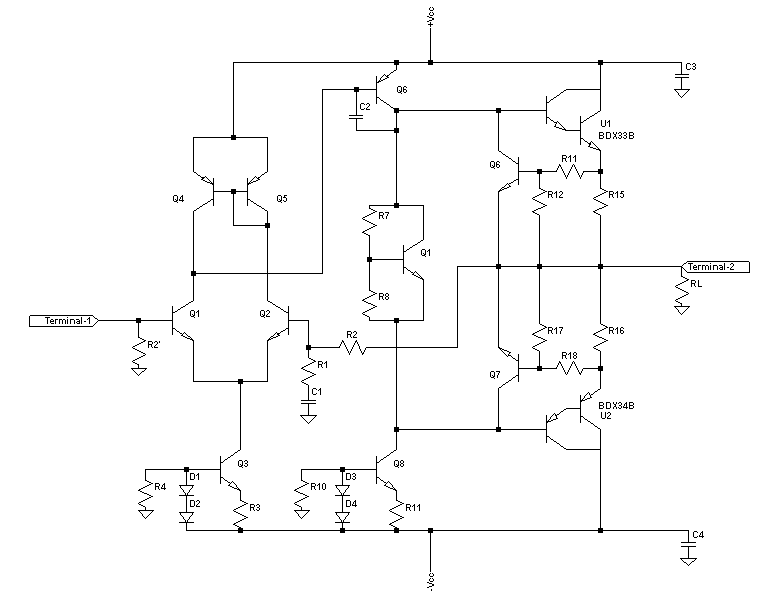
\includegraphics[width=\textwidth]{maalerapporter/effektforstaerker/effektforstaerker_maelerapport.png}
\caption{Effektforstærker med angivelser af terminaler}
\label{fig:testob_efforstaerker}
\end{figure}

\subsection*{Måleopstilling}
Målingerne foretages   ved en opstilling, der laver forstærkning-, frekvensgang- og forvrængningsmåling. Opstillingerne er vist på figur \ref{fig:maaleop-thd}.

\begin{figure}[h]
\centering
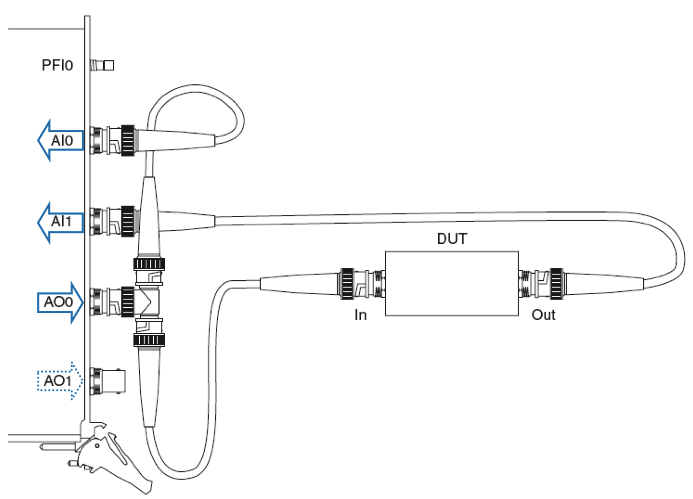
\includegraphics[scale=0.3]{maalerapporter/forforstaerker/maaleopstilling-thd-forforstaerker.png}
\caption{Måleopstilling for forstærkning-, frekvensgang- og forvrængningsmåling \cite{maaling-mm5}}
\label{fig:maaleop-thd}
\end{figure}

\subsection*{Anvendt udstyr}
\begin{table}[h]
\centering
\begin{tabular}{l|c|l}
\hline\hline
Instrument & AAU-nr. & Fabrikant, type m.v. \\
\hline\hline
Oscilloskop & 33851 & Agilent 54621A \\[4pt]
Oscillator & 07997 & B\&O RC-oscillator TG7 \\[4pt]
Spændingsforsyning & 33907& HAMEG HM7042 \\[4pt]
Multimeter & 33048 & Fluke and Philips FLUKE 37 \\[4pt]
Multimeter & 08518 & Fluke and Philips FLUKE 37 \\[4pt]
Effektmodstand 8,2~\ohm & 2159 & Ikke Angivet \\[4pt]
Audioanalysator & 76986 & National Instruments NI-PCI-4461 \\
\hline\hline
\end{tabular}
\label{tab:maaleudstyr_forforstaerker}
\end{table}
\clearpage
\subsection*{Måleprocedure}
Proceduren for forstærkning-, frekvensgang- og forvrængningsmålingen er:

\begin{enumerate}
\item Spændingsforsyningen indstilles $\pm$ 23 V (indstilles med multimeteret) og tilsluttes
\item Testobjektet tilsluttes som på figur \ref{fig:maaleop-thd}
\item Programmet $"$Swept Sine - Linear Response and Harmonic Distortion (DAQmx)$"$ startes
\item $"$Start frequency$"$ under Source settings sættes til 10 Hz
\item $"$Stop frequency$"$ under Source settings sættes til 92 kHz
\item $"$Amplitude$"$ under Source settings sættes til 200 mV
\item $"$THD units$"$ sættes til \%
\item $"$AI Range$"$ for Stimulus channel sættes til $\pm$ 3,16 V
\item $"$AI Range$"$ for Respons channel sættes til $\pm$ 31,6 V
\item $"$Sampling frequency$"$ sættes til 204,8 kHz
\end{enumerate}

Samme procedure gennemføres, hvor amplituden i punkt 6 i stedet sættes til 2 V. Dermed opnåes resultater for både maksimums- og minimumsinput. 


\subsection*{Resultater}
THD, forstærkning og frekvensgang blev målt for effektforstærkeren, resultaterne kan aflæses i figur \ref{fig:apeff:frek200mv} til figur \ref{fig:apeff:thd200mv} 

\begin{figure}[h]
\centering
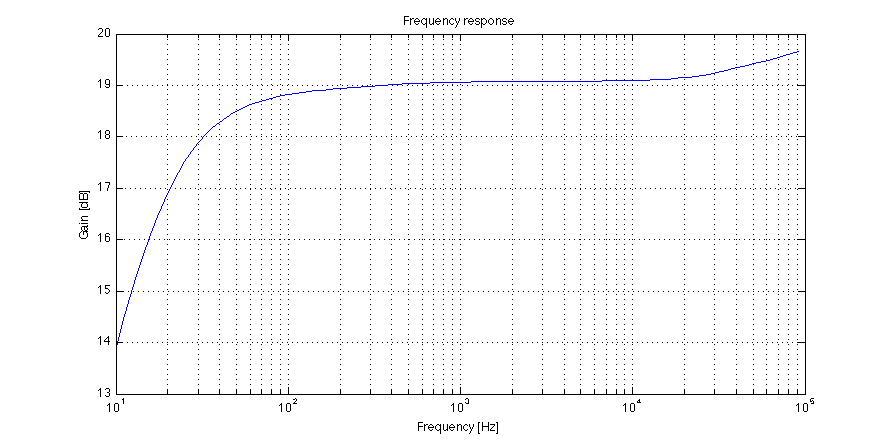
\includegraphics[width=\textwidth]{maalerapporter/effektforstaerker/200mV-45mA-uden-modstand-frek.png}
\caption{Frekvensgangen for effektforstærkeren ved 200 mV.}
\label{fig:apeff:frek200mv}
\end{figure}

\begin{figure}[h]
\centering
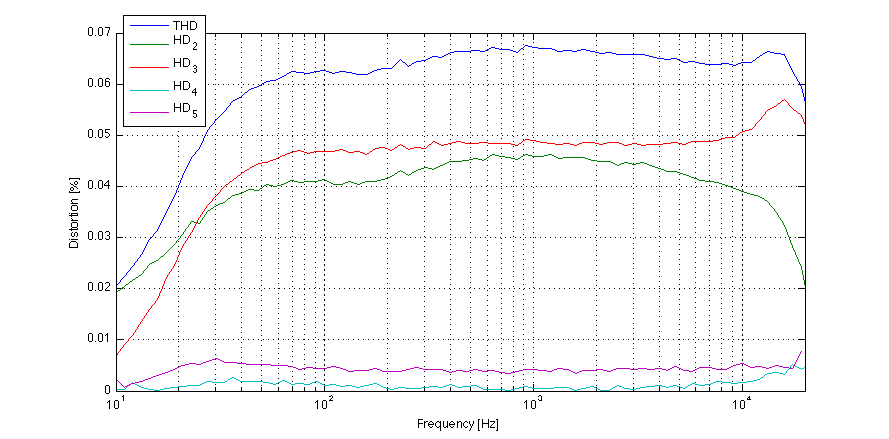
\includegraphics[width=\textwidth]{maalerapporter/effektforstaerker/200mV-45mA-uden-modstand-thd.png}
\caption{THD for effektforstærkeren ved 200 mV.}
\label{fig:apeff:thd200mv}
\end{figure}

\begin{figure}[h]
\centering
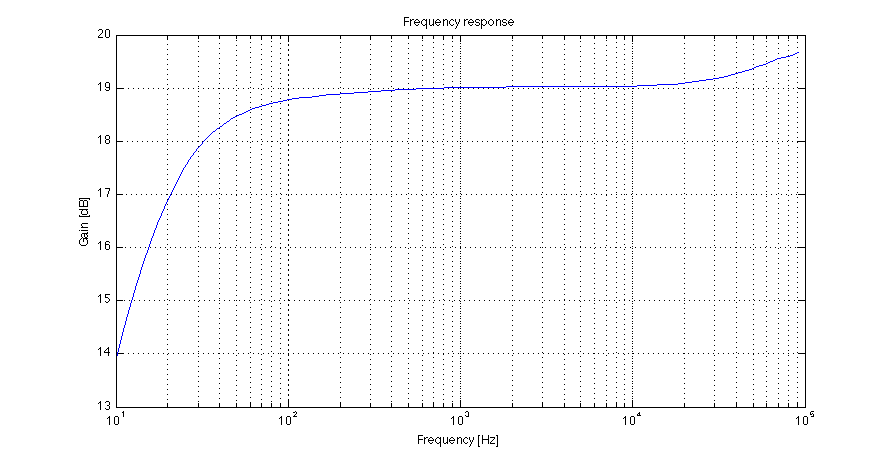
\includegraphics[width=\textwidth]{maalerapporter/effektforstaerker/2V-45mA-uden-modstand-frek.png}
\caption{Frekvensgangen for effektforstærkeren ved 2 V.}
\label{fig:apeff:frek2v}
\end{figure}

\begin{figure}[h]
\centering
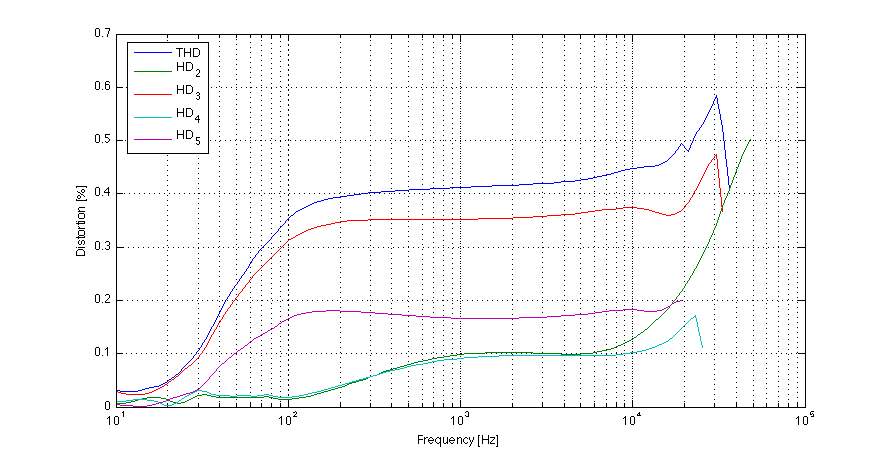
\includegraphics[width=\textwidth]{maalerapporter/effektforstaerker/2V-45mA-uden-modstand-thd.png}
\caption{THD for effektforstærkeren ved 2 V.}
\label{fig:apeff:thd2v}
\end{figure}

%\begin{figure}[h]
%\centering
%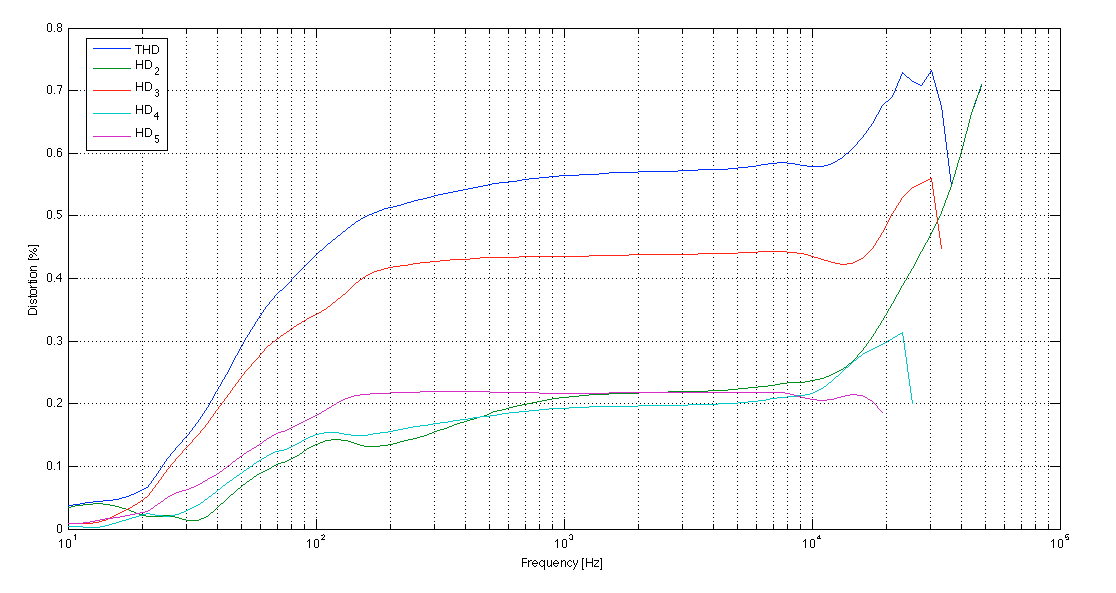
\includegraphics[width=\textwidth]{maalerapporter/effektforstaerker/thd_effekt_fuldudstyring_10min.png}
%\caption{THD for effektforstærkeren ved 2 V  efter maksimal effekt i 10 minutter}
%\label{fig:apeff:thd2v}
%\end{figure}

%\begin{figure}[h]
%\centering
%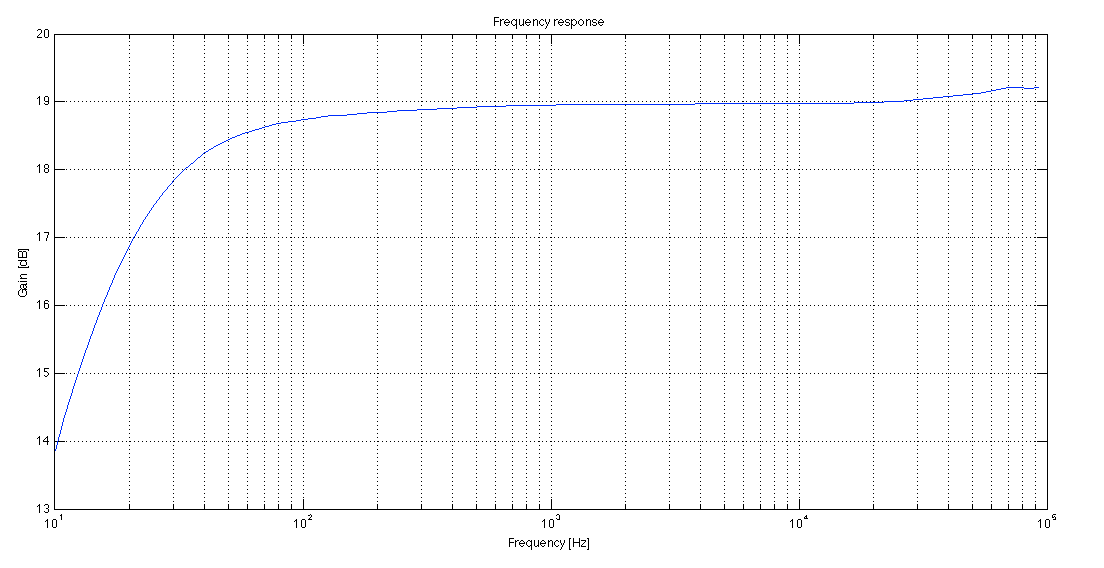
\includegraphics[width=\textwidth]{maalerapporter/effektforstaerker/gain_effekt_fuldudstyring_10min.png}
%\caption{ Frekvensgangen for effektforstærkeren ved 2 V efter maksimal effekt i 10 minutter.}
%\label{fig:apeff:thd2v}
%\end{figure}

%\subsection*{Måleusikkerheder}
%De væsentligste usikkerheder er:
%\begin{itemize}
%\item Komponent tolerancer
%\item Påvirkning fra måleinstrument
%\item Måleinstrument unøjagtighed
%\item Støj, 50 Hz brum
%\item Anden indstråling
%\end{itemize}
%\fixme{Kig på de her fejlkilder, i alle målerapporter}